%Toy example text
%\todo[inline]{I expect to see first the general control problem 13a-13e, then the specific example. This way, if you define once here, we dnot have to worry about re-defining the control problem later. So: here;s the general control problem; here's a simple system.}
%The control problem we solve is a version of \eqref{eq:min rob problem}, using the smooth version of robustness ($\srob$ instead of $\rob$).
%\begin{subequations}
%\label{eq:general_ctrl}
%\begin{align}
%\text{max } & \srob_{\formula}(\sstraj) - \gamma \sum_{k=0}^{N-1} l(x_{k+1},u_{k}) \\
%\text{s.t. } & x_{k+1} = f(x_k,u_k), \, \forall k=0,\dotsc,N-1 \\
% & x_k \in X, \, \forall k=0,\dotsc,N \\
% & u_k \in U, \, \forall k=0,\dotsc,N-1 \\
% & \delta \srob_{\formula}(\sstraj) \geq 0
%\end{align}
%\end{subequations}
%\todo[inline]{stick to $\formula$ for a formula, not $\formula$ (unless there's a good reason)}
%If we set $\gamma=0$ and $\delta=0$, we recover the problem in \eqref{eq:min rob problem} with the smooth robustness in the cost function. In the above formulation, $l(x_{k+1},u_{k})$ is a system specific control cost, e.g. the LQR cost $x_k'Qx_k + u_k'Ru_k$. $X$ and $U$ define constraints on the state $x$ and control $u$ respectively. 
To solve Problem $P_\rob$ given in \eqref{eq:general_ctrl}, we replace the true robustness $\robf$ by its smooth approximation $\srobf$.
We thus obtain Problem $P_{\srob}$.
We illustrate the approach on a simple linear system,
and provide more extensive case studies in Section \ref{sec:case study}.

\subsubsection{Illustrative example}
\label{sec:illustrative example}
We consider a linear system with the following dynamics:
\begin{equation}
\label{eq:PointMass}
x_{k+1} = x_k + u_k
\end{equation}

The specification is 
\[\formula = \always_{[0,20]} \neg (x_k \in \text{Unsafe}) \land \eventually_{[0,20]} (x_k \in \text{Terminal})\]
with the sets $\text{Unsafe}=[-1,1]^2$ i.e. a hyper-cube in $\mathbb{R}^2$ with length 2, centered on the origin) and $\text{Terminal}=[2,2.5]^2$. 
The state space is $X=[-2.5,2.5]^2$, $U=[0.3,0.3]^2$, $\delta=1$, and we optimize for two different values of $\gamma$, $0.1$ and $0.001$. 
The initial point of the optimization is $x_0=[-2,-2]'$. 
The control cost is $l(x_k,u_k) = ||x_k||_{2}^2$, so that $\sum_kl(x_k,u_k)$ penalizes the length of the trajectory. Here, $hrz(\formula) = 21$.

\textbf{Optimization solver.}
We use Sequential Quadratic Programming (SQP) to solve the optimization problem $P_{\srob}$.
SQP solves constrained non-linear optimization problems, like $P_{\srob}$, by creating a sequence of quadratic approximations to the problem and solving these approximate problems.
SQP enjoys various convergence-to-(local)-minima properties, depending on the assumptions we place on the problem. 
See \cite[Section 2.9]{Polak97_Optim}.
For example, for SQP to converge to a strict local minimum (a minimum that is strictly smaller than any objective function value in an open neighborhood around it), it suffices that 
1) all constraint functions be twice Lipschitz continuously differentiable (which is true in our case), and 
2) at points in the search space that lie on the boundary of the inequality-feasible set (where the inequality constraints are satisfied with equality), there exists a search direction towards the interior of the feasible set that does not violate the equality constraints (the so-called Mangasarian-Fromowitz constraint qualification) \cite[Assumption 2.9.1]{Polak97_Optim}.
This is also true in our case since our equality constraints come from the dynamics and are always enforced for any $\mathbf{u}$.

\textbf{Solver initialization}.
To initialize SQP (i.e., give it a starting point for the optimization), we need an \textit{initial trajectory} that starts from $x_0$ and ends in the $\text{Terminal}$ set.
We obtain this initial trajectory the standard way, by solving a feasibility linear program with constraints \eqref{eq:general ctrl dyn}-\eqref{eq:general ctrl U}.
By definition, the solution to a feasibility program is a trajectory that simply satisfies the constraints without optimizing the objective.

\textbf{Results}.
Fig.~\ref{fig:toy control} shows the sets, initial trajectory (which is unsafe and has a robustness of $-1$), and the two trajectories for the two values of $\gamma$. Both trajectories satisfy the specification $\formula$. Intuitively, the trajectories in Fig.\ref{fig:toy control} make sense, as for a higher value of $\gamma=0.1$ we get a shorter trajectory, which is closer to unsafe set, hence satisfies $\formula$ less robustly ($\rob_{\formula}=0.65$) and for a smaller value of $\gamma=0.001$ we get a longer trajectory with a higher robustness ($\rob_{\formula}=1.21$).

\begin{figure}[t]
\centering
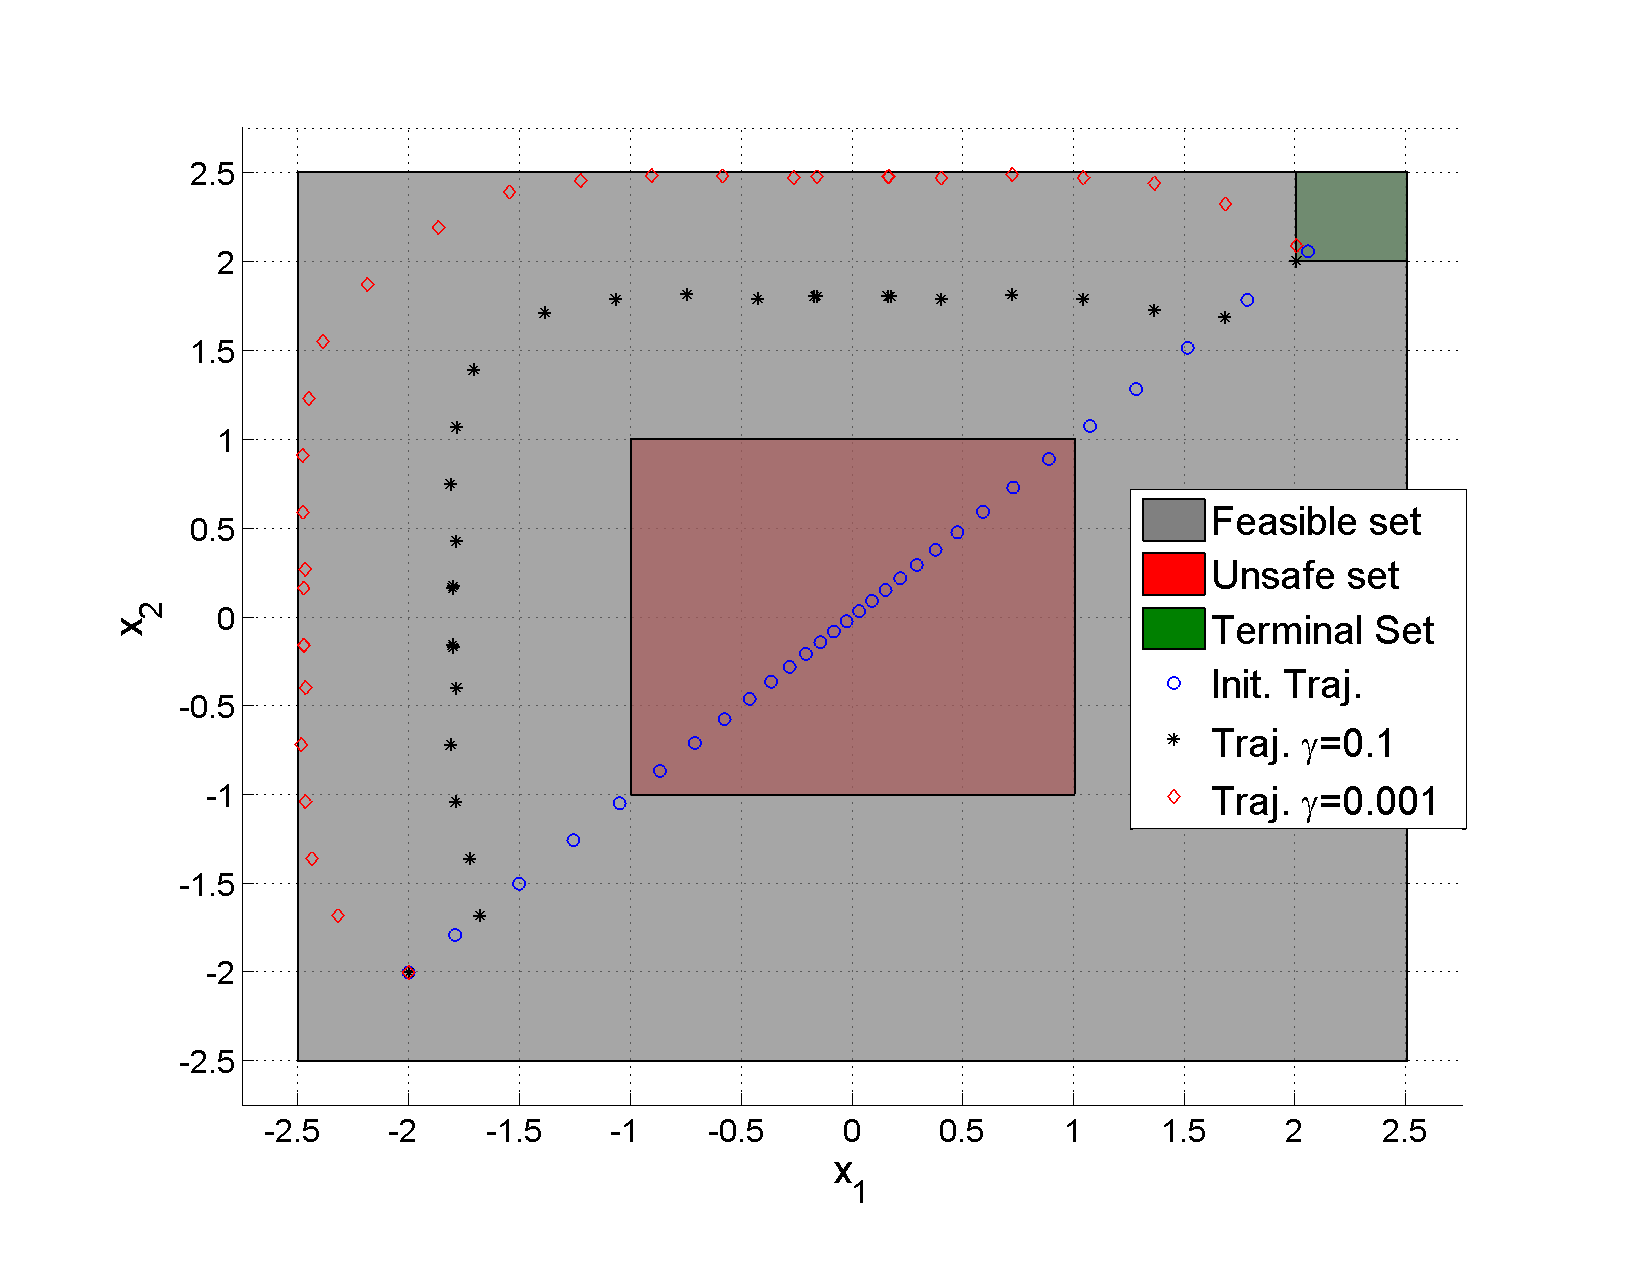
\includegraphics[width=0.49\textwidth]{figures/ToyExampleControl}
\vspace{-30pt}
\caption{{\small Initial trajectory and trajectories obtained for two different values of $\gamma$ in \eqref{eq:general_ctrl}.}}
\label{fig:toy control}
\vspace{-10pt}
\end{figure}